\documentclass[convert]{standalone}

\usepackage{tikz}
\usepackage{graphicx}
\pagestyle{empty}

% INT_AY20_MP3_L22_Fig07_F_mag_dir.tex

\begin{document}
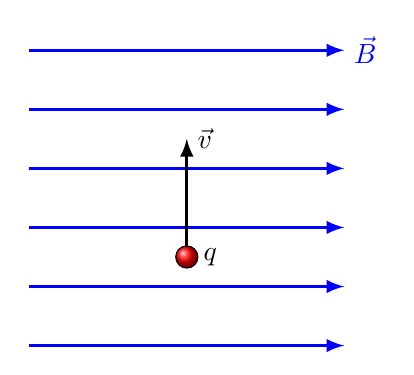
\begin{tikzpicture}

	% Magnetic field lines with label node
	
	\foreach \y in {-1.875, -1.125, ..., 1.875}
		\draw [->, > = latex, very thick, blue] (-2, \y) -- (2, \y);
		
	\node at (2, 1.875) [right, blue] {${\vec B}$};
			
	% Positive charge with velocity vector
	
	\draw [->, > = latex, very thick] (0, -0.75) -- (0, 0.75) node [right] {${\vec v}$};
	\draw [ball color = red] (0, -0.75) circle (4 pt) node [right = 0.25 em] {$q$};
	
\end{tikzpicture}
\end{document}